
This section introduces the HPC application studied in this research and delves into characterizing them. The main source of these applications is the ongoing Exascale Proxy Application Project[cite], commonly known as ECP proxy apps. Along with these proxy apps, Lulesh[cite], another commonly used mini-app in the HPC community, is considered in this study. For characterisation, at first, hostspot analysis is performed using Intel Vtune(2022.3.0) to identify the functions with most execution time. Then, Intel Advisor is used to generate Roofline models to identify the compute-memory intensity of those functions. Table~\ref{table:apps} shows the application names along with the functions and Figure~\ref{fig:roofline} shows the position in the Roofline model.

\begin{figure}[t]%[bp]
\begin{center}
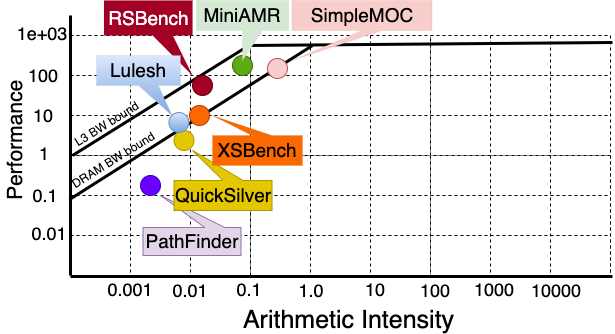
\includegraphics[width=1\linewidth]{MEMSYS22/figures/roofline/roofline_pim.png}
\end{center}
  \vspace{-0.1in}
\caption{Approximate Roofline positioning of the studied functions of different applications.}
\label{fig:roofline}
\vspace{-0.2in}
\end{figure}



\subsection{SimpleMOC}
The main computation function in SimpleMOC is the $attenuate\_fluxes$  which is a memory bound kernel (see Fig.~\ref{fig:roof-simplemoc}). 


%./PathFinder.x -x ../data/scaleData/1kx750.adj_list
\subsection{PathFinder}
The main computation function in PathFinder is the $findAndRecordAllPaths$  which is a memory bound kernel (see Fig.~\ref{fig:roof-simplemoc}). 




\subsection{XSBench}
The main computation function in XSBench is the $calculate_micro_xs$  which is a memory bound kernel. 

\subsection{RSBench}
The main computation function in XSBench is the $calculate_micro_xs$  which is a memory bound kernel. 


\subsection{MiniAMR}
The main computation function in miniAMR is the $stencil\_calc$  which is a memory bound kernel (see Fig.~\ref{fig:roof-miniamr}). 

\subsection{Lulesh}
Two functions in Lulesh is in our interest. 1). CalcFBHourglassForce (highest time consuming but hihger AI) and 2). CalcElemCharacteristicLength (yellow but lowest AI)

CalcKinematicsForElems



%./qs --nParticles=10000
\subsection{Quicksilver}
macroscopicCrossSection

%
%
\begin{table}[b]
%\normalsize
\small
\caption{HPC Benchmarks and their Memory-Bound/Critical Kernel/Functions identified}
\centering
%    \begin{tabularx}{\columnwidth}{lcc}
    \begin{tabularx}{\columnwidth}{ccc}
    %\begin{tabularx}{7.2cm}{lcc}
\toprule
    % \hline
    Bechmarks & Function & Memory/compute bound \\
\midrule
%jacobi & - & +++ \\
%laplace  & - & +++ \\

%Lulesh-2 & CalcElemCharacteristicLength & DRAM BW bound \\
SimpleMOC & attenuate\_fluxes & DRAM BW bound \\
PathFinder   & findAndRecordAllPaths & DRAM BW bound \\
XSBench      & calculate\_micro\_xs & DRAM BW bound \\
RSBench      & c_mul & L3 BW bound \\
MiniAMR      & stencil\_calc & L3 BW bound \\
QuickSilver      & macroscopicCrossSection & DRAM BW bound \\
Lulesh & CalcKinematicsForElems & DRAM BW bound \\
\bottomrule
   \end{tabularx}
\label{table:apps}
%\vspace{-0.5cm}
\end{table}
%
%
%
%\begin{figure}[t!]
%\centering
%\includegraphics[width=\columnwidth]{figure/processor.png}
%\caption{Schematic view of the Next Generation Microprocessor~(NGMP)}
%\label{fig:processor}
%%\vspace{-0.4cm}
%\end{figure}



%-	Roofline model \\
%-	Identifying functions that are memory intensive \\


%\subsection{Jacobi}
%The main function in Jacobi is the $stencil\_jacobi$ function which is a memory bound kernel (see Fig.~\ref{fig:roof-jacobi}). 







%\begin{figure}[t!]
%\centering
%\includegraphics[width=70mm, height= 50mm]{figure/pmtj.pdf}
%%\vspace{.5em} 
%\caption{STT-MRAM cell}
%%\vspace{-1.5em} 
%\label{fig:pmtj}
%%\vspace{-0.3cm}   
%\end{figure} 
%
%
%
%
%  
%\looseness -1
%
%
%
%\begin{figure}[t!]
%\centering
%\includegraphics[width=\columnwidth]{figure/DeviceCapacity.pdf}
%%\vspace{.5em} 
%\caption{DRAM and STT-MRAM capacity growth in years} %\pr{23-Feb: Kazi, do we have any data from after 2016? Take care of this only if you have some extra time. }}
%%\vspace{-1.5em} 
%\label{fig:Capa}
%\vspace{-0.3cm}  
%\end{figure}  


%\begin{figure}[t]%[bp]
%\begin{center}
%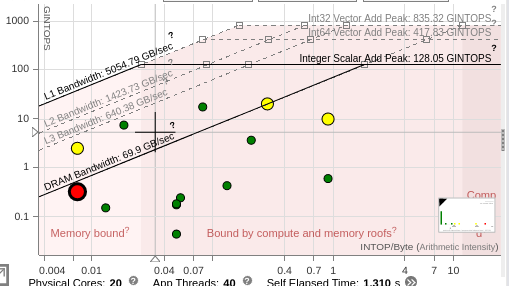
\includegraphics[width=1\linewidth]{MEMSYS22/figures/roofline/pathfinder.png}
%\end{center}
%  \vspace{-0.1in}
%\caption{Positioning of the main compute kernel of PathFinder app in Roofline. Here the red circle indicates the $findAndRecordAllPaths$ function }
%\label{fig:roof-pathfinder}
%\vspace{-0.2in}
%\end{figure}

%\begin{figure}[t]%[bp]
%\begin{center}
%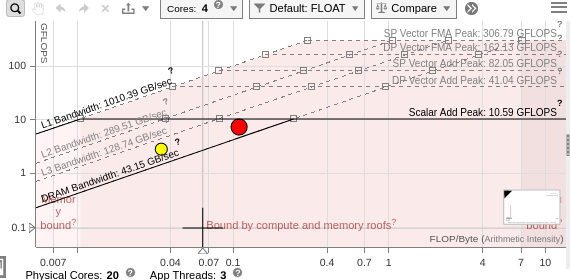
\includegraphics[width=1\linewidth]{MEMSYS22/figures/roofline/miniamr.png}
%\end{center}
%  \vspace{-0.1in}
%\caption{Positioning of the main compute kernel of MiniAMR app in Roofline. Here the red circle indicates the $stencil\_calc$ function }
%\label{fig:roof-miniamr}
%\vspace{-0.2in}
%\end{figure}



%\begin{figure}[h]%[bp]
%\begin{center}
%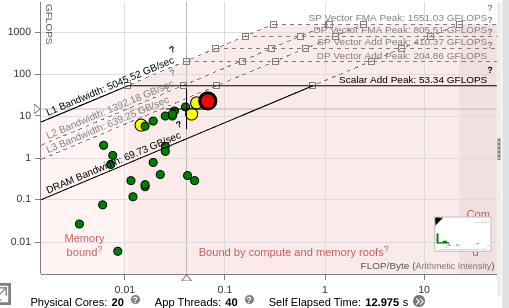
\includegraphics[width=1\linewidth]{MEMSYS22/figures/roofline/simplesoc.png}
%\end{center}
%  \vspace{-0.1in}
%\caption{Positioning of the main compute kernel of SimpleMOC app in Roofline. Here the red circle indicates the $attenuate\_fluxes$ function }
%\label{fig:roof-simplemoc}
%\vspace{-0.2in}
%\end{figure}